\documentclass[border=90pt]{standalone}

\usepackage{graphicx}
\usepackage{tikz}
\usetikzlibrary{calc,patterns,angles,quotes}
\usepackage{fancyhdr}
\usepackage{hyperref}
\usepackage{chemfig}
\usepackage{enumitem}
\usepackage{placeins}
\usepackage{caption}
\usepackage{array}
\usepackage{float}
\usepackage{amsmath, amssymb, amscd, MnSymbol,mathrsfs}
\usepackage{tcolorbox}
\usepackage{bibref}
\usepackage{bm}
\newcommand{\vect}[1]{\boldsymbol{\mathbf{#1}}}
\usepackage{pdfpages}

\usepackage{empheq}
\usepackage{pgfplots}
\pgfplotsset{compat=1.18}
\usepackage[oldvoltagedirection]{circuitikz}
\usepackage{booktabs}
\usepackage{array}
\usepackage{arydshln}
\usepackage{tcolorbox}

\usepackage{hyperref}
\usepackage{cancel}
\usepackage{changepage}
\usepackage{placeins}
\usepackage{enumitem}
\usepackage{pgf}
\usetikzlibrary{decorations.markings}
\usetikzlibrary{decorations.pathmorphing}
\usepackage{tikz-3dplot}
\usetikzlibrary{hobby}
\usepackage{microtype}

\usepackage{soul}
\usepackage[normalem]{ulem} % [normalem] prevents the package from changing the default behavior of `\emph` to underline.

\def\las{0.74}

\begin{document}
        
    \begin{tikzpicture}[use Hobby shortcut]
        \def\width{4}
        \def\gap{8}
        \def\main{6}
        \def\curvy{1.9}
        
        \def\n{3.3}
        \def\z{1/\n}
        \pgfmathsetmacro{\s}{1-\z}
        
        \coordinate (A) at (0,\main);
        \coordinate (B) at (\width*\z-\width*\z*0.23,\main+\curvy-\curvy*0.7);
        \coordinate (C) at (\width*\z,\main+\curvy);
        
        \coordinate (A2) at (\width,\main);
        \coordinate (B2) at (\width*\s+\width*\z*0.23,\main+\curvy-\curvy*0.7);
        \coordinate (C2) at (\width*\s,\main+\curvy);
        
        \coordinate (A3) at (0,\main+\gap);
        \coordinate (B3) at (\width*\z-\width*\z*0.23,\main+\gap-\curvy+\curvy*0.7);
        \coordinate (C3) at (\width*\z,\main+\gap-\curvy);
        
        \coordinate (A4) at (\width,\main+\gap);
        \coordinate (B4) at (\width*\s+\width*\z*0.23,\main+\gap-\curvy+\curvy*0.7);
        \coordinate (C4) at (\width*\s,\main+\gap-\curvy);
        \pgfmathsetmacro\k{(-2.3+\width*1/4)/2}
        \pgfmathsetmacro\kt{\width}
        
        \draw[-] (\width*1/4,\main+\curvy) -- (-2.3,\main+\curvy);
        \draw[-] (\width*1/4,\main-\curvy+\gap) -- (-2.3,\main-\curvy+\gap);
        \draw[thick, {Latex[length=3.5mm,width=3.5mm]}-{Latex[length=3.5mm,width=3.5mm]}, line width=0.01cm] (\k,\main-\curvy+\gap) -- (\k,\main+\curvy);
        \draw[-] (C) -- (C2);
        \draw[-] (C3) -- (C4);
        \draw[fill=white,white] (\k-0.4,10.6) rectangle (\k+0.4,9);
        \node[fill=white] at (\k,10.1) {\textsf{\textbf{G\kern-0.07em A\kern-0.07em U\kern-0.07em G\kern-0.07em E L\kern-0.07em E\kern-0.07em N\kern-0.07em G\kern-0.07em T\kern-0.07em H}}};
        \node[fill=white] at (\k,9.65) {\textsf{\textbf{\textls[0] 5\kern-0.07em 0\kern-0.07em M\kern-0.07em M}}};
        \draw[-,line width=0.4mm] (\k-0.5,9.35)--(\k+0.5,9.35);
        \draw[-,line width=0.4mm] (\k-0.45,9.25)--(\k+0.45,9.25);
        \draw[hobby,tension=3] (A) .. (B) .. (C);
        \draw[hobby,tension=3] (A2) .. (B2) .. (C2);
        \draw[hobby,tension=3] (A3) .. (B3) .. (C3);
        \draw[hobby,tension=3] (A4) .. (B4) .. (C4);
        \draw[-] (\width*\z,\main+\curvy) -- (\width*\z,\main+\gap-\curvy);
        \draw[-] (\width*\s,\main+\curvy) -- (\width*\s,\main+\gap-\curvy);
        \draw[-] (0,0) -- (\width,0);
        \draw[-] (0,0) -- (0,\main);
        \draw[-] (\width,0) -- (\width,\main);
        \draw[-] (0,\main+\gap) -- (0,2*\main+\gap);
        \draw[-] (0,2*\main+\gap) -- (\width,2*\main+\gap);
        \draw[-] (\width,2*\main+\gap) -- (\width,\main+\gap);
        \node at (\kt,10.2) {\textsf{\textbf{W\kern-0.07em I\kern-0.07em D\kern-0.07em T\kern-0.07em H =}}};
        \node at (\kt+0.35,9.6) {\textsf{\textbf{T\kern-0.07em H\kern-0.07em I\kern-0.07em C\kern-0.07em K\kern-0.07em N\kern-0.07em E\kern-0.07em S\kern-0.07em S =}}};
        \draw [line width=2.1pt, line cap=round, dash pattern=on 0pt off 1.7\pgflinewidth] (\kt+1,10.05) -- (\kt+2.9,10.05);
        \draw [line width=2.1pt, line cap=round, dash pattern=on 0pt off 1.7\pgflinewidth] (\kt+1.7,9.46) -- (\kt+2.9,9.46);

        \node at (\width*0.5,2*\gap+\width-1) {\Huge \textrm{\textbf{AR}}};        
                \Large

        \node at (\width*0.5,-2) {\textsf{\textbf{VICKERS}}};
        \node at (\width*0.5,-2-\las) {\textsf{\textbf{HARDNESS}}};

        \node at (\width*0.5,-2-2*\las) {\textsf{\phantom{36, 36.8} \textbf{HV5}}};        
        \draw [line width=2.1pt, line cap=round, dash pattern=on 0pt off 1.7\pgflinewidth] (\width*0.5-1.5,-2.2-2*\las) -- (\width*0.5+0.4,-2.2-2*\las);        
        \node at (\width*0.5,-2-3*\las) {\textsf{\textbf{AS RECEIVED}}};
        \node at (\width*0.5,-2-4*\las) {\phantom{{{PRECIPITATION HARDENED AT 184 DEGREES.}}}};
        
    \end{tikzpicture}\hspace{13em}
    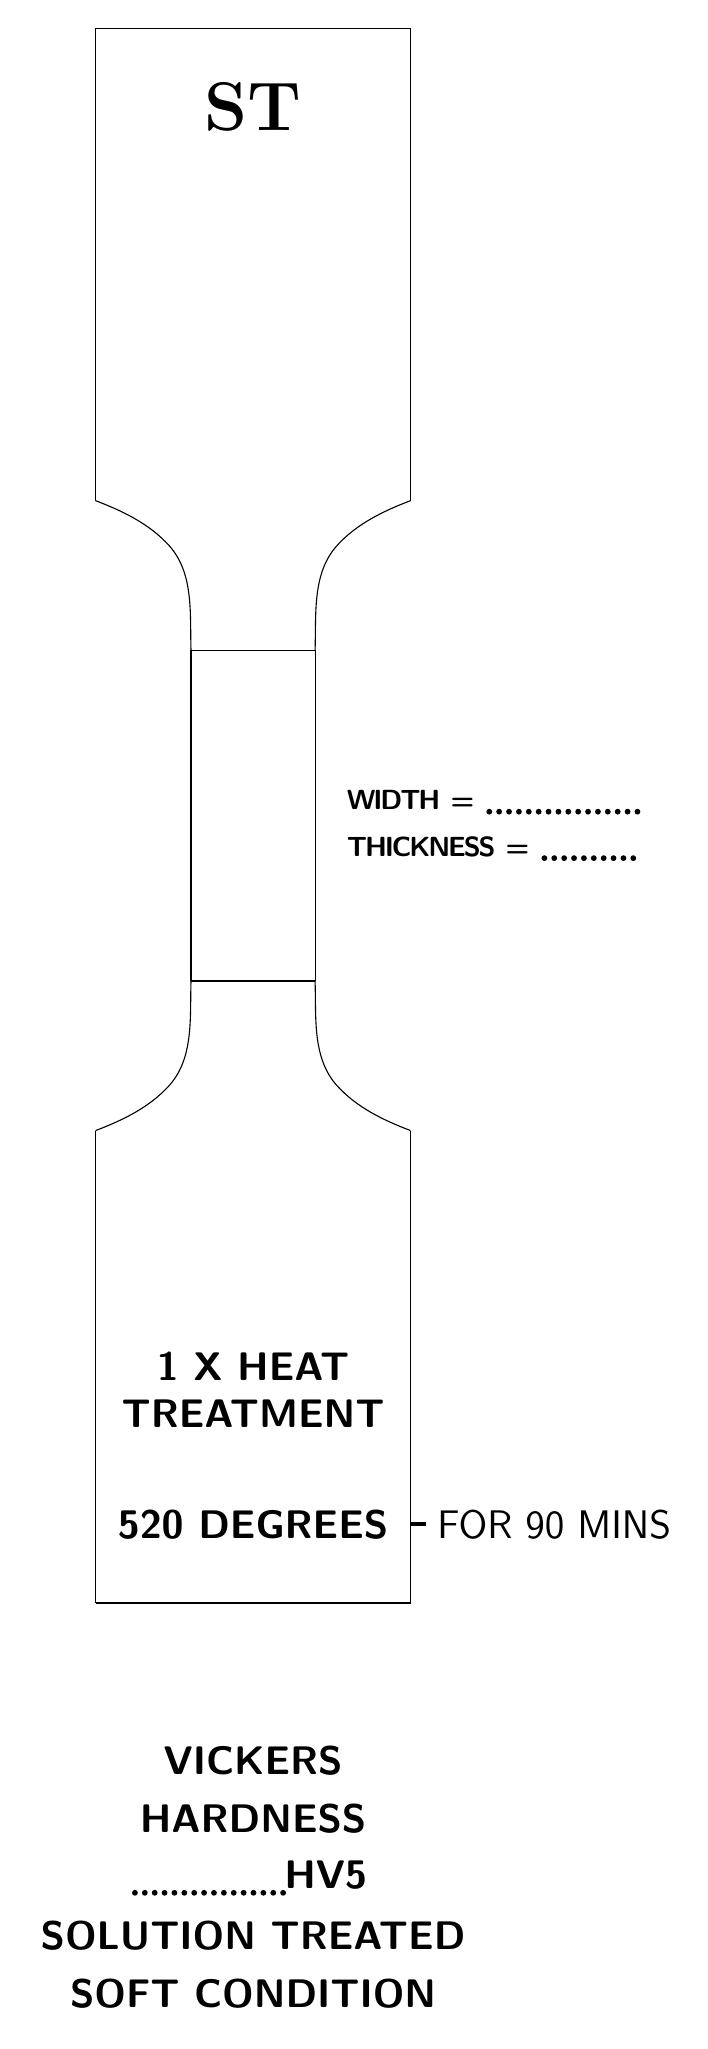
\begin{tikzpicture}[use Hobby shortcut]
        \def\width{4}
        \def\gap{8}
        \def\main{6}
        \def\curvy{1.9}
        
        \def\n{3.3}
        \def\z{1/\n}
        \pgfmathsetmacro{\s}{1-\z}
        
        \coordinate (A) at (0,\main);
        \coordinate (B) at (\width*\z-\width*\z*0.23,\main+\curvy-\curvy*0.7);
        \coordinate (C) at (\width*\z,\main+\curvy);
        
        \coordinate (A2) at (\width,\main);
        \coordinate (B2) at (\width*\s+\width*\z*0.23,\main+\curvy-\curvy*0.7);
        \coordinate (C2) at (\width*\s,\main+\curvy);
        
        \coordinate (A3) at (0,\main+\gap);
        \coordinate (B3) at (\width*\z-\width*\z*0.23,\main+\gap-\curvy+\curvy*0.7);
        \coordinate (C3) at (\width*\z,\main+\gap-\curvy);
        
        \coordinate (A4) at (\width,\main+\gap);
        \coordinate (B4) at (\width*\s+\width*\z*0.23,\main+\gap-\curvy+\curvy*0.7);
        \coordinate (C4) at (\width*\s,\main+\gap-\curvy);
        \pgfmathsetmacro\k{(-2.3+\width*1/4)/2}
        \pgfmathsetmacro\kt{\width}
        
        \draw[-] (C) -- (C2);
        \draw[-] (C3) -- (C4);
        \draw[hobby,tension=3] (A) .. (B) .. (C);
        \draw[hobby,tension=3] (A2) .. (B2) .. (C2);
        \draw[hobby,tension=3] (A3) .. (B3) .. (C3);
        \draw[hobby,tension=3] (A4) .. (B4) .. (C4);
        \draw[-] (\width*\z,\main+\curvy) -- (\width*\z,\main+\gap-\curvy);
        \draw[-] (\width*\s,\main+\curvy) -- (\width*\s,\main+\gap-\curvy);
        \draw[-] (0,0) -- (\width,0);
        \draw[-] (0,0) -- (0,\main);
        \draw[-] (\width,0) -- (\width,\main);
        \draw[-] (0,\main+\gap) -- (0,2*\main+\gap);
        \draw[-] (0,2*\main+\gap) -- (\width,2*\main+\gap);
        \draw[-] (\width,2*\main+\gap) -- (\width,\main+\gap);
        \node at (\kt,10.2) {\textsf{\textbf{W\kern-0.07em I\kern-0.07em D\kern-0.07em T\kern-0.07em H =}}};
        \node at (\kt+0.35,9.6) {\textsf{\textbf{T\kern-0.07em H\kern-0.07em I\kern-0.07em C\kern-0.07em K\kern-0.07em N\kern-0.07em E\kern-0.07em S\kern-0.07em S =}}};
        \draw [line width=2.1pt, line cap=round, dash pattern=on 0pt off 1.7\pgflinewidth] (\kt+1,10.05) -- (\kt+2.9,10.05);
        \draw [line width=2.1pt, line cap=round, dash pattern=on 0pt off 1.7\pgflinewidth] (\kt+1.7,9.46) -- (\kt+2.9,9.46);
        \node at (\width*0.5,2*\gap+\width-1) {\Huge \textrm{\textbf{ST}}};
        
        \node at (\width*0.5,3) {\Large \textsf{\textbf{1 X HEAT}}};
        \node at (\width*0.5,2.4) {\Large \textsf{\textbf{TREATMENT}}};
        \node at (\width*0.5,1) {\Large \textsf{\textbf{520 DEGREES}}};
        
        \draw[line width=0.5mm] (\width,1) -- (\width+0.2,1) node[right] {\Large \textsf{FOR 90 MINS}};
        \Large
        \node at (\width*0.5,-2) {\textsf{\textbf{VICKERS}}};
        \node at (\width*0.5,-2-\las) {\textsf{\textbf{HARDNESS}}};
        \node at (\width*0.5,-2-2*\las) {\textsf{\phantom{36, 36.8} \textbf{HV5}}};        
        \draw [line width=2.1pt, line cap=round, dash pattern=on 0pt off 1.7\pgflinewidth] (\width*0.5-1.5,-2.2-2*\las) -- (\width*0.5+0.4,-2.2-2*\las);
        \node at (\width*0.5,-2-3*\las) {\textsf{\textbf{SOLUTION TREATED}}};
        \node at (\width*0.5,-2-4*\las) {\textsf{\textbf{SOFT CONDITION}}};

        
    \end{tikzpicture}\hspace{2em}
    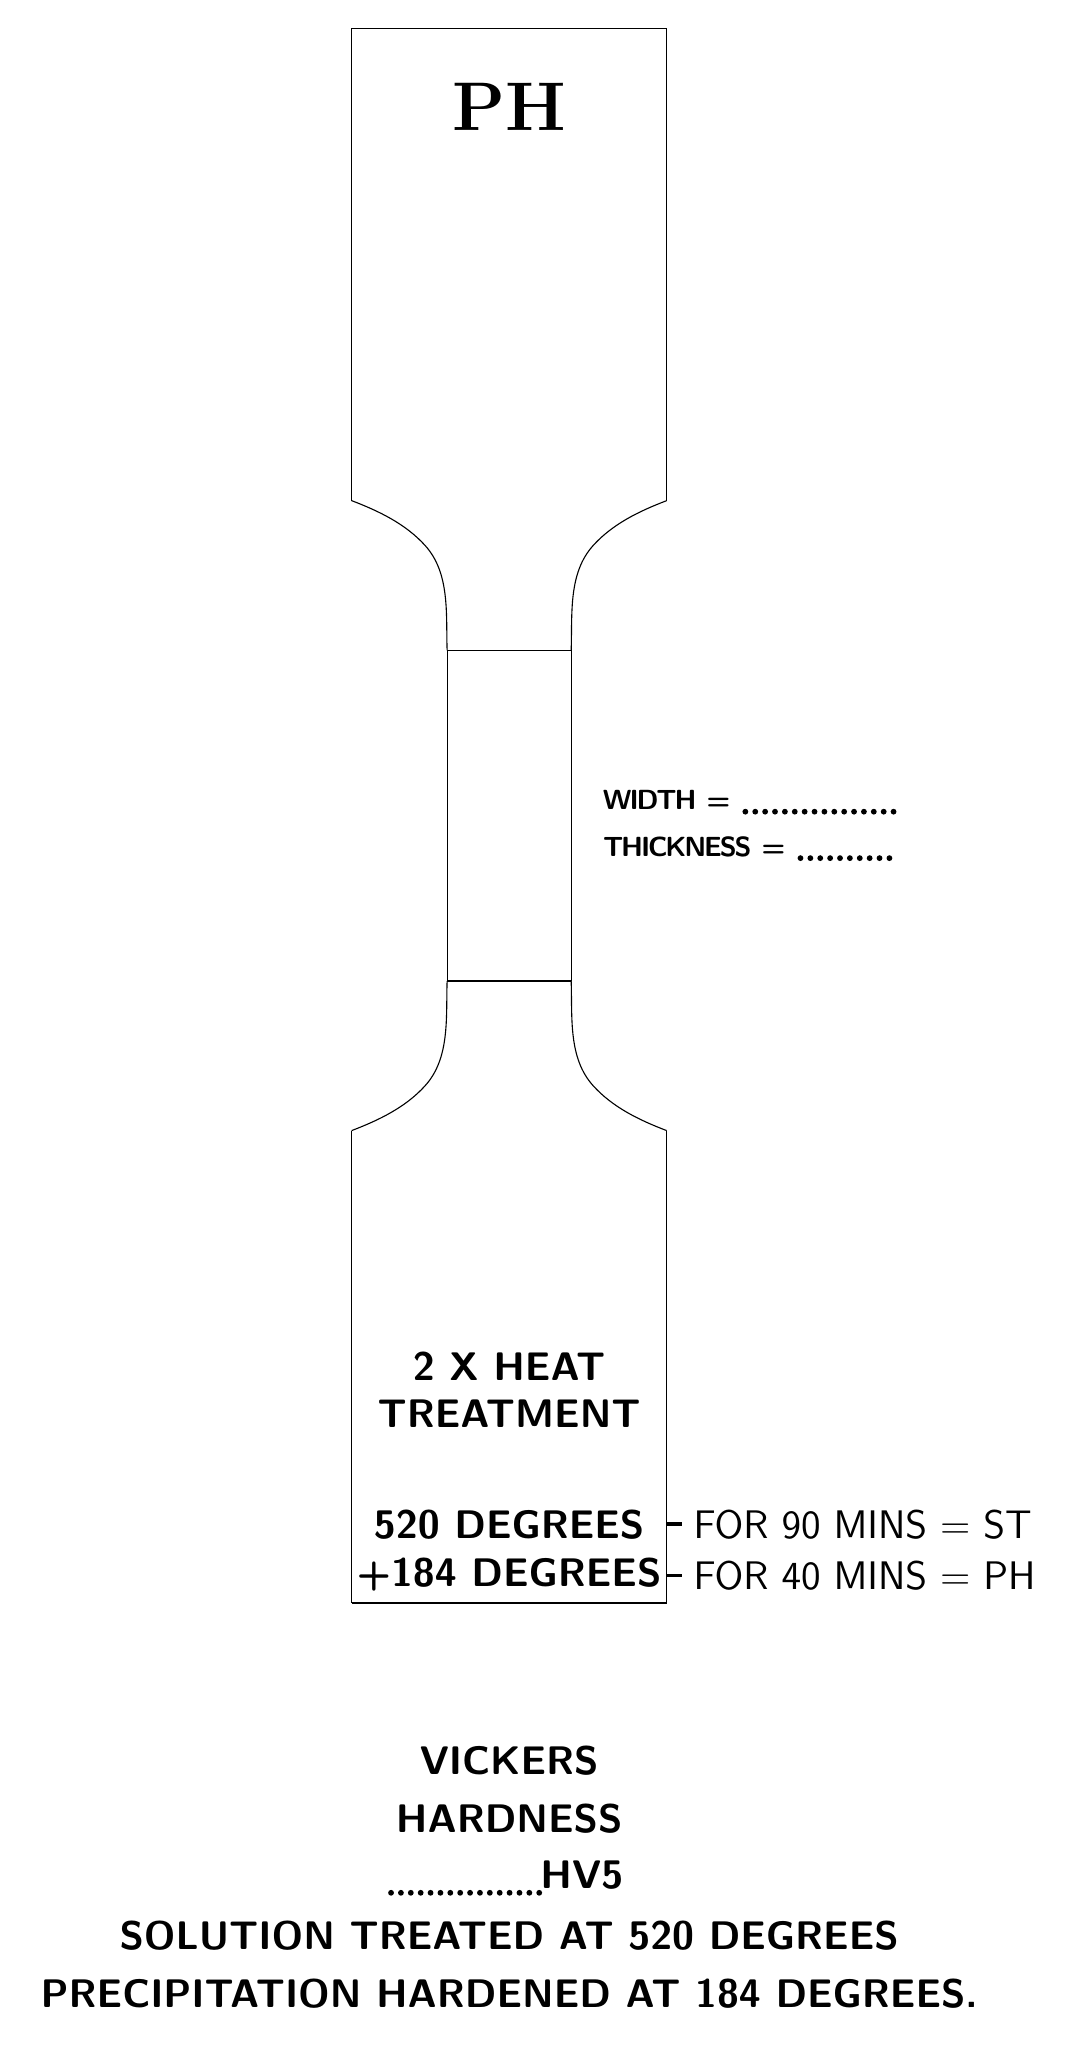
\begin{tikzpicture}[use Hobby shortcut]
        \def\width{4}
        \def\gap{8}
        \def\main{6}
        \def\curvy{1.9}
        
        \def\n{3.3}
        \def\z{1/\n}
        \pgfmathsetmacro{\s}{1-\z}
        
        \coordinate (A) at (0,\main);
        \coordinate (B) at (\width*\z-\width*\z*0.23,\main+\curvy-\curvy*0.7);
        \coordinate (C) at (\width*\z,\main+\curvy);
        
        \coordinate (A2) at (\width,\main);
        \coordinate (B2) at (\width*\s+\width*\z*0.23,\main+\curvy-\curvy*0.7);
        \coordinate (C2) at (\width*\s,\main+\curvy);
        
        \coordinate (A3) at (0,\main+\gap);
        \coordinate (B3) at (\width*\z-\width*\z*0.23,\main+\gap-\curvy+\curvy*0.7);
        \coordinate (C3) at (\width*\z,\main+\gap-\curvy);
        
        \coordinate (A4) at (\width,\main+\gap);
        \coordinate (B4) at (\width*\s+\width*\z*0.23,\main+\gap-\curvy+\curvy*0.7);
        \coordinate (C4) at (\width*\s,\main+\gap-\curvy);
        \pgfmathsetmacro\k{(-2.3+\width*1/4)/2}
        \pgfmathsetmacro\kt{\width}
        
        \draw[-] (C) -- (C2);
        \draw[-] (C3) -- (C4);
        \draw[hobby,tension=3] (A) .. (B) .. (C);
        \draw[hobby,tension=3] (A2) .. (B2) .. (C2);
        \draw[hobby,tension=3] (A3) .. (B3) .. (C3);
        \draw[hobby,tension=3] (A4) .. (B4) .. (C4);
        \draw[-] (\width*\z,\main+\curvy) -- (\width*\z,\main+\gap-\curvy);
        \draw[-] (\width*\s,\main+\curvy) -- (\width*\s,\main+\gap-\curvy);
        \draw[-] (0,0) -- (\width,0);
        \draw[-] (0,0) -- (0,\main);
        \draw[-] (\width,0) -- (\width,\main);
        \draw[-] (0,\main+\gap) -- (0,2*\main+\gap);
        \draw[-] (0,2*\main+\gap) -- (\width,2*\main+\gap);
        \draw[-] (\width,2*\main+\gap) -- (\width,\main+\gap);
        \node at (\kt,10.2) {\textsf{\textbf{W\kern-0.07em I\kern-0.07em D\kern-0.07em T\kern-0.07em H =}}};
        \node at (\kt+0.35,9.6) {\textsf{\textbf{T\kern-0.07em H\kern-0.07em I\kern-0.07em C\kern-0.07em K\kern-0.07em N\kern-0.07em E\kern-0.07em S\kern-0.07em S =}}};

        \draw [line width=2.1pt, line cap=round, dash pattern=on 0pt off 1.7\pgflinewidth] (\kt+1,10.05) -- (\kt+2.9,10.05);
        \draw [line width=2.1pt, line cap=round, dash pattern=on 0pt off 1.7\pgflinewidth] (\kt+1.7,9.46) -- (\kt+2.9,9.46);

        \node at (\width*0.5,2*\gap+\width-1) {\Huge \textrm{\textbf{PH}}};
        
        \node at (\width*0.5,3) {\Large \textsf{\textbf{2 X HEAT}}};
        \node at (\width*0.5,2.4) {\Large \textsf{\textbf{TREATMENT}}};
        \node at (\width*0.5,1) {\Large \textsf{\textbf{520 DEGREES}}};
        \node at (\width*0.5,0.35) {\Large \textsf{\textbf{+184 DEGREES}}};
        \draw[line width=0.5mm] (\width,1) -- (\width+0.2,1) node[right] {\Large \textsf{FOR 90 MINS = ST}};
        \draw[line width=0.5mm] (\width,0.35) -- (\width+0.2,0.35) node[right] {\Large \textsf{FOR 40 MINS = PH}};
        
        \Large
        \node at (\width*0.5,-2) {\textsf{\textbf{VICKERS}}};
        \node at (\width*0.5,-2-\las) {\textsf{\textbf{HARDNESS}}};
        \node at (\width*0.5,-2-2*\las) {\textsf{\phantom{36, 36.8} \textbf{HV5}}};        
        \draw [line width=2.1pt, line cap=round, dash pattern=on 0pt off 1.7\pgflinewidth] (\width*0.5-1.5,-2.2-2*\las) -- (\width*0.5+0.4,-2.2-2*\las);
        \node at (\width*0.5,-2-3*\las) {\textsf{\textbf{SOLUTION TREATED AT 520 DEGREES}}};
        \node at (\width*0.5,-2-4*\las) {\textsf{\textbf{PRECIPITATION HARDENED AT 184 DEGREES.}}};
        
    \end{tikzpicture}
    
\end{document}